\documentclass[10pt]{article}
\usepackage[margin=0.62in]{geometry}
\usepackage{amsmath,amssymb,enumitem,xcolor,tikz,fancyvrb,fontspec}
\usetikzlibrary{arrows.meta,cd,positioning}
\pagestyle{empty}
\setlist{nosep,leftmargin=1.35em}
\definecolor{priority}{RGB}{125,25,35}
\newfontfamily\leanfont{DejaVu Sans}
\newenvironment{lean}{\Verbatim[fontsize=\scriptsize,frame=single,framesep=2mm,formatcom=\leanfont]}{\endVerbatim}
\newcommand{\idim}{\operatorname{idim}}
\newcommand{\Mod}{\mathbf{Mod}}
\newcommand{\high}{\textcolor{priority}{\textbf{High}}}
\newcommand{\med}{\textbf{Medium}}
\newcommand{\low}{\textbf{Low}}
\begin{document}
\begin{center}
{\Large\bfseries Re-audit: injective dimension in \texttt{ModuleCat}}\\[-1mm]
\small Lean/API design, categorical pattern, and proof-shape review
\end{center}
\small
\section*{Verdict}
The dimension-shifting argument is coherent: embed into an injective, identify the two cokernels,
and induct. The universe bridge is also a sensible implementation of a genuinely cross-universe
statement. I would request two cleanups (dead code and misleading section placement), then approve.
The strongest follow-up is not another local simplification: it is reusable transport API for exact
equivalences and semilinear quotients.

\section*{Findings, with quoted code}

\subsection*{1. Remove the dead elaboration line --- \high}
\begin{lean}
have := exactS.hasInjectiveDimensionLT_X₃_iff n inferInstance
apply (exactS.hasInjectiveDimensionLT_X₃_iff n inferInstance).symm.trans
  ((ih e).trans (exactS'.hasInjectiveDimensionLT_X₃_iff n inferInstance))
\end{lean}
The anonymous \texttt{have} is unused, and the identical expression is
built on the next line. Delete it. Prefer \texttt{exact} rather than \texttt{apply} here because the
entire proposition is supplied:
\begin{lean}
exact (exactS.hasInjectiveDimensionLT_X₃_iff n inferInstance).symm.trans
  ((ih eCoker).trans
    (exactS'.hasInjectiveDimensionLT_X₃_iff n inferInstance))
\end{lean}

\subsection*{2. Move the linear auxiliary lemma out of the ring-equivalence section --- \high}
\begin{lean}
variable [Small.{v} R] {R' : Type u'} [CommRing R'] (e : R ≃+* R')

lemma hasInjectiveDimensionLE_iff_of_linearEquiv_aux
    {M : ModuleCat.{v} R} {N : ModuleCat.{max v v'} R}
    (e : M ≃ₗ[R] N) (n : ℕ) : ...
\end{lean}
This lemma uses neither \texttt{R'} nor the ring equivalence from the section. Lean omits unused
section parameters from the generated declaration, so this is not a theorem-signature bug; it is a
source-structure and readability problem. It also makes the inner \texttt{e} shadow the outer
\texttt{e}. Give this lemma its own section and use names such as \texttt{eMN} and \texttt{eCoker}.

\subsection*{3. Fix and strengthen the module documentation --- \high}
The original diff's heading says:
\begin{lean}
# Projective Dimension in ModuleCat
\end{lean}
It must say \texttt{Injective Dimension}. Add one terse scope sentence: the file proves invariance of
\texttt{HasInjectiveDimensionLE} and \texttt{injectiveDimension} under linear and ring-semilinear
equivalences, including differing universes. This makes the unusual universe machinery discoverable.

\subsection*{4. Factor semilinear equivalences on quotients --- \med}
\begin{lean}
let eCoker : ModuleCat.of R (I / f.range) ≃ₛₗ[RingHomClass.toRingHom e]
    ModuleCat.of R' (I' / f'.hom.range) := {
  __ := Submodule.mapQ _ _ eI.toLinearMap
    (by simp [← eqmap, Submodule.map_equiv_eq_comap_symm])
  invFun := Submodule.mapQ _ _ eI.symm.toLinearMap
    (by simp [← eqmap, ← Submodule.map_le_iff_le_comap])
  left_inv x := Submodule.Quotient.induction_on _ x (by simp)
  right_inv x := Submodule.Quotient.induction_on _ x (by simp) }
\end{lean}
This is correct-looking but low-level and broadly reusable. The existing same-ring
\texttt{Submodule.Quotient.equiv} pattern suggests adding its semilinear analogue: a semilinear
equivalence plus equality of mapped submodules induces an equivalence of quotients. Then this block
becomes one constructor call, and inverse proofs stop obscuring dimension shifting.

\subsection*{5. Package the repeated ``mono to cokernel short exact sequence'' --- \med}
\begin{lean}
let S : ShortComplex (ModuleCat.{v} R) :=
  ModuleCat.shortComplexOfCompEqZero _ _
    f.exact_map_mkQ_range.linearMap_comp_eq_zero
have exactS := ModuleCat.shortComplex_shortExact S
  f.exact_map_mkQ_range injf (Submodule.mkQ_surjective _)
\end{lean}
The proof repeats this shape for \texttt{f} and \texttt{f'}. A helper returning the canonical short
exact sequence
\(0\to M\xrightarrow f I\to I/\operatorname{range}(f)\to0\)
from \texttt{Function.Injective f} would remove bookkeeping and expose the mathematical step. If such
a helper belongs in the short-complex API, put it there rather than locally in this file.

\subsection*{6. Name local instances and evidence --- \med}
\begin{lean}
have : Module.Injective R' I' :=
  Module.injective_module_of_injective_object R' I'
...
have : Injective (ModuleCat.of R I) := by
  rw [← Module.injective_iff_injective_object]
  exact Module.Injective.of_ringEquiv e.symm eI.symm
\end{lean}
Anonymous typeclass evidence works, but names such as \texttt{injI'} and \texttt{injI} make later
\texttt{inferInstance} calls auditable and avoid fragility if another proposition of the same shape is
introduced. Also consider writing \texttt{Injective I} if it elaborates definitionally; the extra
\texttt{ModuleCat.of R I} visually suggests a second object even though \texttt{I} is already a
\texttt{ModuleCat} object.

\subsection*{7. Improve names at the equality boundary --- \low}
\begin{lean}
refine eq_of_forall_ge_iff (fun N => ?_)
induction N with
\end{lean}
Here \texttt{N} already denotes a module in the theorem statement. Rename the extended-natural cutoff
to \texttt{d} or \texttt{k}. Likewise avoid three meanings of \texttt{e}: ring equivalence, module
equivalence, and quotient equivalence. Suggested vocabulary: \texttt{eR}, \texttt{eMN},
\texttt{eI}, \texttt{eCoker}.

\subsection*{8. Keep the universe bridge; make its purpose explicit --- \low}
\begin{lean}
let eM : M \simeq_l[R] ModuleCat.of R (ULift.{v'} M) :=
  ULift.moduleEquiv.symm
let eN : N \simeq_l[R'] ModuleCat.of R' (ULift.{v} N) :=
  ULift.moduleEquiv.symm
rw [hasInjectiveDimensionLE_iff_of_linearEquiv_aux eM,
  hasInjectiveDimensionLE_iff_of_linearEquiv_aux eN]
\end{lean}
This is a good pattern: normalize both objects into \(\max(v,v')\), apply the same-universe theorem,
and transport back. Do not collapse it into opaque coercion tricks. A short comment saying
``move both modules to a common universe'' is justified here.

\subsection*{9. Local options and instances are correctly scoped --- positive}
\begin{lean}
set_option backward.isDefEq.respectTransparency.types false in
attribute [local instance] RingHomInvPair.of_ringEquiv in
lemma hasInjectiveDimensionLE_iff_of_semiLinearEquiv_aux ...
\end{lean}
The narrow \texttt{in} scope is preferable to changing global elaboration behavior. Keep this shape.
If later API removes the elaboration workaround, delete the option rather than broadening its scope.

\subsection*{10. Preserve the thin public specialization --- positive}
\begin{lean}
lemma injectiveDimension_eq_of_linearEquiv (e : M ≃ₗ[R] N) :
    injectiveDimension M = injectiveDimension N :=
  injectiveDimension_eq_of_semiLinearEquiv.{v, v'}
    (M := M) (N := N) (RingEquiv.refl R) e
\end{lean}
This is good API layering: the linear theorem is a one-line specialization of the stronger semilinear
theorem, not a duplicated proof. Keep it. The explicit universe arguments and named module arguments
are justified here because they document which two universe levels are being related.

\subsection*{11. Check imports with the project linter --- \low}
\begin{lean}
public import Mathlib.Algebra.Category.ModuleCat.Ext.DimensionShifting
public import Mathlib.Algebra.Category.ModuleCat.EnoughInjectives
public import Mathlib.Algebra.Category.ModuleCat.Injective
public import Mathlib.Algebra.Homology.ShortComplex.ModuleCat
public import Mathlib.CategoryTheory.Abelian.Injective.Dimension
\end{lean}
Several may be transitively available, but do not guess from this review: run Mathlib's
minimum-import/lint workflow on the target branch and retain only direct conceptual dependencies.
The explicit imports are otherwise clear.

\section*{Big idea: categorical transport, not module-level reconstruction}
The proof manually realizes an equivalence of module categories induced by \(e:R\simeq R'\).
Conceptually, an exact equivalence of abelian categories preserves injectives, short exact sequences,
and therefore injective dimension. A reusable theorem should have the shape
\[
 F:C\simeq D,\quad F\text{ exact}
 \quad\Longrightarrow\quad
 \idim(X)=\idim(FX).
\]
The current theorem then becomes an application to the module-category equivalence associated to a
ring equivalence. This would eliminate most of the transported injective and quotient construction:
\begin{lean}
have : Injective (ModuleCat.of R I) := by
  rw [← Module.injective_iff_injective_object]
  exact Module.Injective.of_ringEquiv e.symm eI.symm
...
let eCoker : ModuleCat.of R (I / f.range) \simeq_sl[...] ... := { ... }
\end{lean}
This is a follow-up design direction, not a blocker: developing the exact-equivalence theorem may be
larger than this PR.

\begin{center}
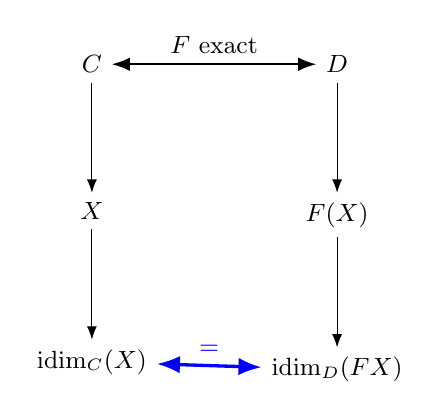
\begin{tikzpicture}[>=Latex,node distance=14mm and 26mm,every node/.style={font=\small}]
\node (C) {$C$}; \node[right=of C] (D) {$D$};
\draw[<->,thick] (C) -- node[above] {$F$ exact} (D);
\node[below=of C] (X) {$X$}; \node[below=of D] (FX) {$F(X)$};
\draw[->] (C) -- (X); \draw[->] (D) -- (FX);
\node[below=of X] (dx) {$\idim_C(X)$};
\node[below=of FX] (dfx) {$\idim_D(FX)$};
\draw[->] (X) -- (dx); \draw[->] (FX) -- (dfx);
\draw[<->,very thick,blue] (dx) -- node[above] {$=$} (dfx);
\end{tikzpicture}
\end{center}

\section*{Current induction, made visible}
\begin{center}
\begin{tikzcd}[column sep=1.35em,row sep=2.2em]
0 \arrow[r] & M \arrow[r,"f"] \arrow[d,"e'"',"\sim"] & I \arrow[r] \arrow[d,"e_I"',"\sim"] & C \arrow[r] \arrow[d,"e_C"',"\sim"] & 0 \\
0 \arrow[r] & N \arrow[r,"f'"] & I' \arrow[r] & C' \arrow[r] & 0
\end{tikzcd}
\end{center}
\[
\idim(M)\le n+1
\iff \idim(C)\le n
\iff \idim(C')\le n
\iff \idim(N)\le n+1.
\]
This is the right proof invariant. Refactoring should preserve this visible four-step chain.

\section*{Proposed order of action}
\begin{enumerate}
\item Delete the unused \texttt{have}; correct the title.
\item Isolate the linear auxiliary section and remove shadowing names.
\item Add a semilinear quotient-equivalence constructor, if acceptable in scope.
\item Optionally package the canonical short exact sequence for an injective linear map.
\item Treat exact-equivalence invariance as a separate categorical follow-up.
\end{enumerate}

\section*{Verification note}
This audit project is pinned to an older Mathlib snapshot than the supplied diff: several quoted APIs
are unavailable locally. Therefore this document reviews the submitted source and proof architecture;
it does not claim a local compilation of that newer patch. The review artifact itself was compiled to
PDF.
\end{document}
